% this file is called up by thesis.tex
% change according to folder and file names
\ifpdf
    \graphicspath{{6/figures/PNG/}{6/figures/PDF/}{6/figures/}}
\else
    \graphicspath{{6/figures/EPS/}{6/figures/}}
\fi

%: ----------------------- contents from here ------------------------
% content in this file will be fed into the main document

\chapter{Βελτιστοποίηση Περιφερειακής Πτερύγωσης Συμπιεστή} % top level followed by section, % ---------------------------------------------------------------------------
Στόχος αυτού του κεφαλαίου είναι η βελτιστοποίηση της περιφερειακής πτερύγωσης συμπιεστή που βρίσκεται εγκατεστημένη στο ΕΘΣ/ΕΜΠ. Η πτερύγωση σχεδιάστηκε από τη \english{SNECMA} και έχει, στο παρελθόν, χρησιμοποιηθεί για τη μελέτη της ροής σε πτερυγώσεις με ακτινικό διάκενο (σχήμα \ref{res:ntua_blade:blade}) για υψηλούς αριθμούς \english{Mach} \footnote{\english{
European project «Advanced Civil Core Compressor Aerodynamics», AER2-CT92-0039, 1/1/1993-30/9/1996.}}. Παρουσίαση της διάταξης υπάρχει στο πλήρες κείμενο της διατριβής.  
   
\begin{figure}[h!]
\centering
  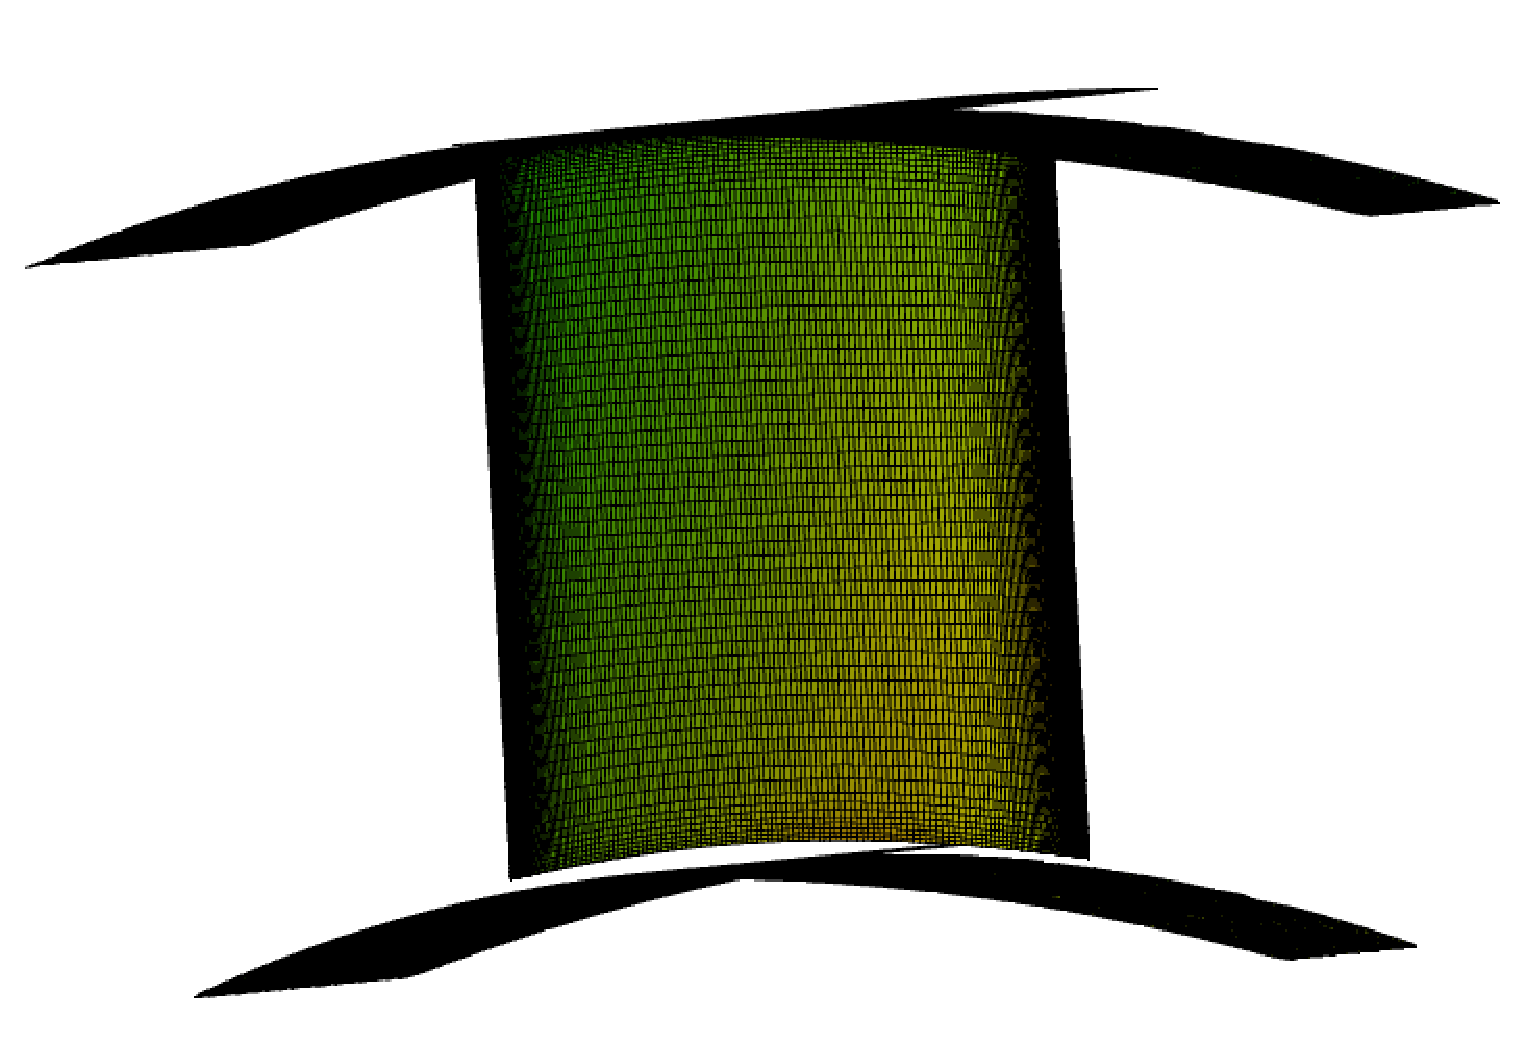
\includegraphics[width=.5\textwidth]{blade.eps}
  \caption{Βελτιστοποίηση περιφερειακής πτερύγωσης συμπιεστή: Τα πτερύγια στηρίζονται στο εξωτερικό κέλυφος (\english{shroud}) ενώ  το ακτινικό διάκενο δημιουργείται στην «επαφή» με το εσωτερικό κέλυφος (\english{hub}). Ο λόγος ακτίνων των δύο κελυφών είναι $R_{hub}/R_{shroud}=0.75$.}
  \label{res:ntua_blade:blade}
\end{figure}

Το πρόβλημα βελτιστοποίησης του σχήματος της (σταθερής κατά την ακτινική κατεύθυνση) αεροτομής του πτερυγίου αντιμετωπίζεται ως πρόβλημα μονοκριτηριακής βελτιστοποίησης  με περιορισμούς ελάχιστου πάχους σε τρεις θέσεις της αεροτομής, στο  $30\%$, $60\%$ και $90\%$ της χορδής. Το ελάχιστο αποδεκτό πάχος σε κάθε θέση καθορίζεται στο $90\%$ του αντίστοιχου πάχους του υπάρχοντος σχεδιασμού. Επιπλέον, επιβάλλεται περιορισμός ως προς τη μέση γωνία εξόδου ροής ($\alpha_2<53^o$). Η μελέτη έγινε για ακτινικό διάκενο ίσο με το $2\%$ του μήκους της χορδής.    

Η βελτιστοποίηση πραγματοποιήθηκε έχοντας ως μοναδική προς ελαχιστοποί-ηση συνάρτηση κόστους το μέσο συντελεστή απωλειών ολικής πίεσης $PLC_{av}$.  Η ποσότητα $PLC_{av}$ ορίζεται ως η μέση τιμή των τιμών του αντίστοιχου συντελεστή $PLC(r)$ σε κάθε ακτίνα ($r$) ανάμεσα στα δύο κελύφη. Η τελευταία δίνεται από τη σχέση 
\begin{equation}
PLC(r)=\frac{p_{t,inl}-p_t(r)}{p_{t,inl}-p_{inl}}
\label{res:ntua_blade:plc}
\end{equation}

Στο εν λόγω πρόβλημα σχεδιασμού, μιας και η αεροτομή του πτερυγίου διατηρεί-ται σταθερή σε όλες τις ακτινικές θέσεις, απαιτείται αποκλειστικά η παραμετροποίηση μιας 2Δ αεροτομής. Αυτή γίνεται με χρήση πολυωνύμων $NURBS$. Για κάθε πλευρά της αεροτομής υπάρχουν $5$ ελεύθερα σημεία ελέγχου ($10$ μεταβλητές σχεδιασμού). 
Συνολικά, οι άγνωστοι του προβλήματος βελτιστοποίησης είναι $N=20$. 
Αυτά α-ντιστοιχούν σε $5$ σημεία ελέγχου με $2$ ελεύθερες συνιστώσες για κάθε πλευρά της
αεροτομής.

Οι συνθήκες που επιβλήθηκαν στον επιλύτη των εξισώσεων της ροής είναι: (α) για την είσοδο, η περιφερειακή και ακτινική κατανομή της ολικής πίεσης και ολικής θερμοκρασίας και των γωνιών της
ροής αλλά και η ένταση της τύρβης (1.5\%) και (β) για την έξοδο, η τιμή της στατικής πίεσης στην ακτίνα ποδός. Μέσω της εξίσωσης
ακτινικής ισορροπίας,  υπολογίζεται επαναληπτικά η ακτινική κατανομή της στατικής πίεσης σε όλη τη διατομή εξόδου.

Με οικείο λογισμικό, σε κάθε υποψήφια λύση δημιουργείται ένα μη-δομημένο υβριδικό πλέγμα, της τάξης των $600 000$ κόμβων. Η αξιολόγηση κάθε υποψήφιας λύσης γίνεται από επιλύτη των εξισώσεων \english{Navier-Stokes}, με μοντέλο τύρβης αυτό των  \english{Spalart-Allmaras}  και συναρτήσεις τοίχου.  



\section{Αποτελέσματα - Συγκρίσεις } 
Πραγματοποιήθηκαν δύο τρεξίματα βελτιστοποίησης χάριν σύγκρισης. Η μια χρησιμοποιώντας τον προϋπάρχοντα ΜΑΕΑ και η δεύτερη τον προτεινόμενου Μ(\english{PCA})-ΑΕΑ(\english{PCA}). Κατά την εφαρμογή του προϋπάρχοντος ΜΑΕΑ, η φάση της ΠΠΑ ξεκινά όταν στη βάση δεδομένων του ΜΑΕΑ υπάρχουν περισσότερα από $220$ ήδη αξιολογηθέντα άτομα. Αντίθετα, όταν χρησιμοποιείται ο Μ(\english{PCA})ΑΕΑ(\english{PCA}), λόγω της χρήσης της ΑσΚΣ κατά την εκπαίδευση των μεταπροτύπων (μείωση των εισόδων του μεταπροτύπου από $20$ σε $10$), η φάση ΠΠΑ ξεκινά νωρίτερα, όταν στη βάση δεδομένων υπάρχουν μόνο $150$ άτομα. Οι πορείες σύγκλισης των δύο μεθόδων συγκρίνο-νται στο σχήμα \ref{PCAcomp}. Παρατηρείται ότι, κάνοντας χρήση του  Μ(\english{PCA})ΑΕΑ(\english{PCA}), εντοπίζεται ο βέλτιστος σχεδιασμός σε περίπου $250$ αξιολογήσεις ενώ με τον προϋπάρχοντα ΜΑΕΑ χρειάζονται περίπου $450$. Η επίδραση της χρήσης της ΑσΚΣ κατά την εκπαίδευση των μεταπροτύπων στην  ποιότητα των προβλέψεων τους γίνεται εμφανής στο σχήμα \ref{PCAcomp2}. 



\begin{figure}[h!]
\begin{minipage}[b]{0.5\linewidth}
 \centering
 \resizebox*{8cm}{!}{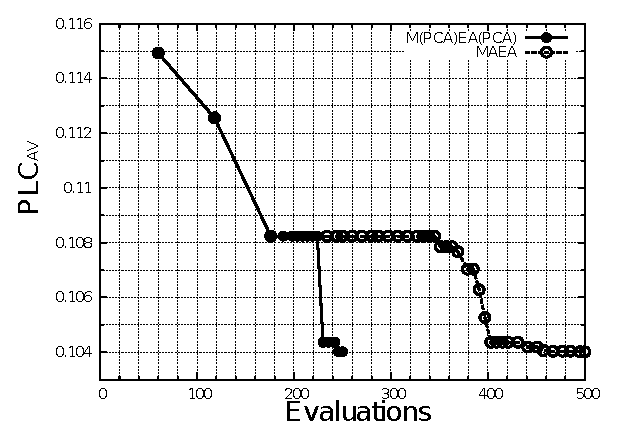
\includegraphics{Comp.eps}}
\end{minipage}
\begin{minipage}[b]{0.5\linewidth}
 \centering
 \resizebox*{4.5cm}{!}{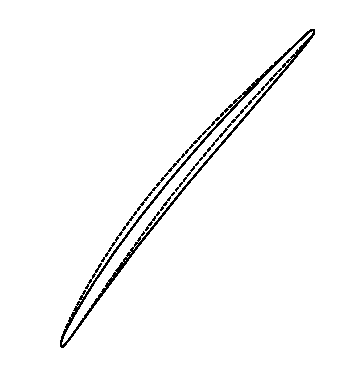
\includegraphics{ntua_foils.eps}}
\end{minipage}
\caption{Βελτιστοποίηση περιφερειακής πτερύγωσης συμπιεστή: Αριστερά: Πορείες σύγκλισης για τον ΜΑΕΑ και τον προτεινόμενο Μ(\english{PCA})ΑΕΑ(\english{PCA}). Δεξιά: Η βέλτιστη αεροτομή, που προέκυψε από τον Μ(\english{PCA})ΑΕΑ(\english{PCA}) (συνεχής γραμμή) και η υπάρχουσα αεροτομή της πειραματικής εγκατάστασης στο ΕΘΣ/ΕΜΠ (διακεκομμένη γραμμή).} 
\label{PCAcomp}
\end{figure}

\begin{figure}[h!]
\begin{minipage}[b]{1\linewidth}
 \centering
 \resizebox*{9cm}{!}{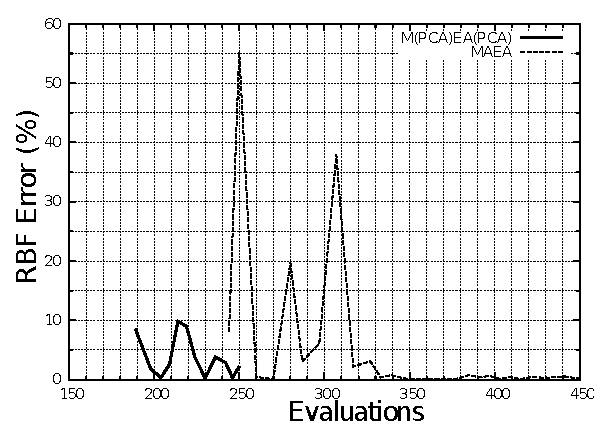
\includegraphics{Comp2.eps}}
\end{minipage}
\caption{Βελτιστοποίηση περιφερειακής πτερύγωσης συμπιεστή: Σύγκριση λάθους πρόβλεψης του μεταπροτύπου (δίκτυα \english{RBF}) κατά την πορεία της εξέλιξης.} 
\label{PCAcomp2}
\end{figure}
\newpage
Η βέλτιστη αεροτομή (σχήμα \ref{PCAcomp}), όπως αυτή εντοπίστηκε από τον \linebreak Μ(\english{PCA})ΑΕΑ(\english{PCA}) έχει μέσες απώλειες πίεσης $PLC_{av}=0.104$, μέση γωνία εξόδου $\alpha_2=52.6^o$ και ικανοποιεί όλους τους τεθέντες περιορισμούς πάχους.


%\begin{figure}[h!]
%\centering
%  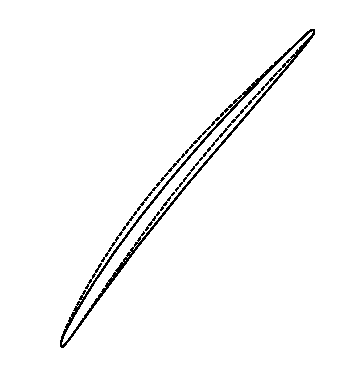
\includegraphics[width=.5\textwidth]{ntua_foils.eps}
%  \caption{Η βέλτιστη αεροτομή (εικόνα %\ref{res:ntua_blade:final}), όπως αυτή σχεδιάστηκε από τον Μ(\english{PCA})ΑΕΑ(\english{PCA}) (συνεχείς γραμμή) και η αρχική αεροτομή (διακεκομμένη γραμμή).}
%  \label{res:ntua_blade:final}
%\end{figure}

%Finally the pressure contour of the optimal blade is presented in figure \ref{res:ntua_blade:Optimal}.

%\begin{figure}[h!]
%\centering
%  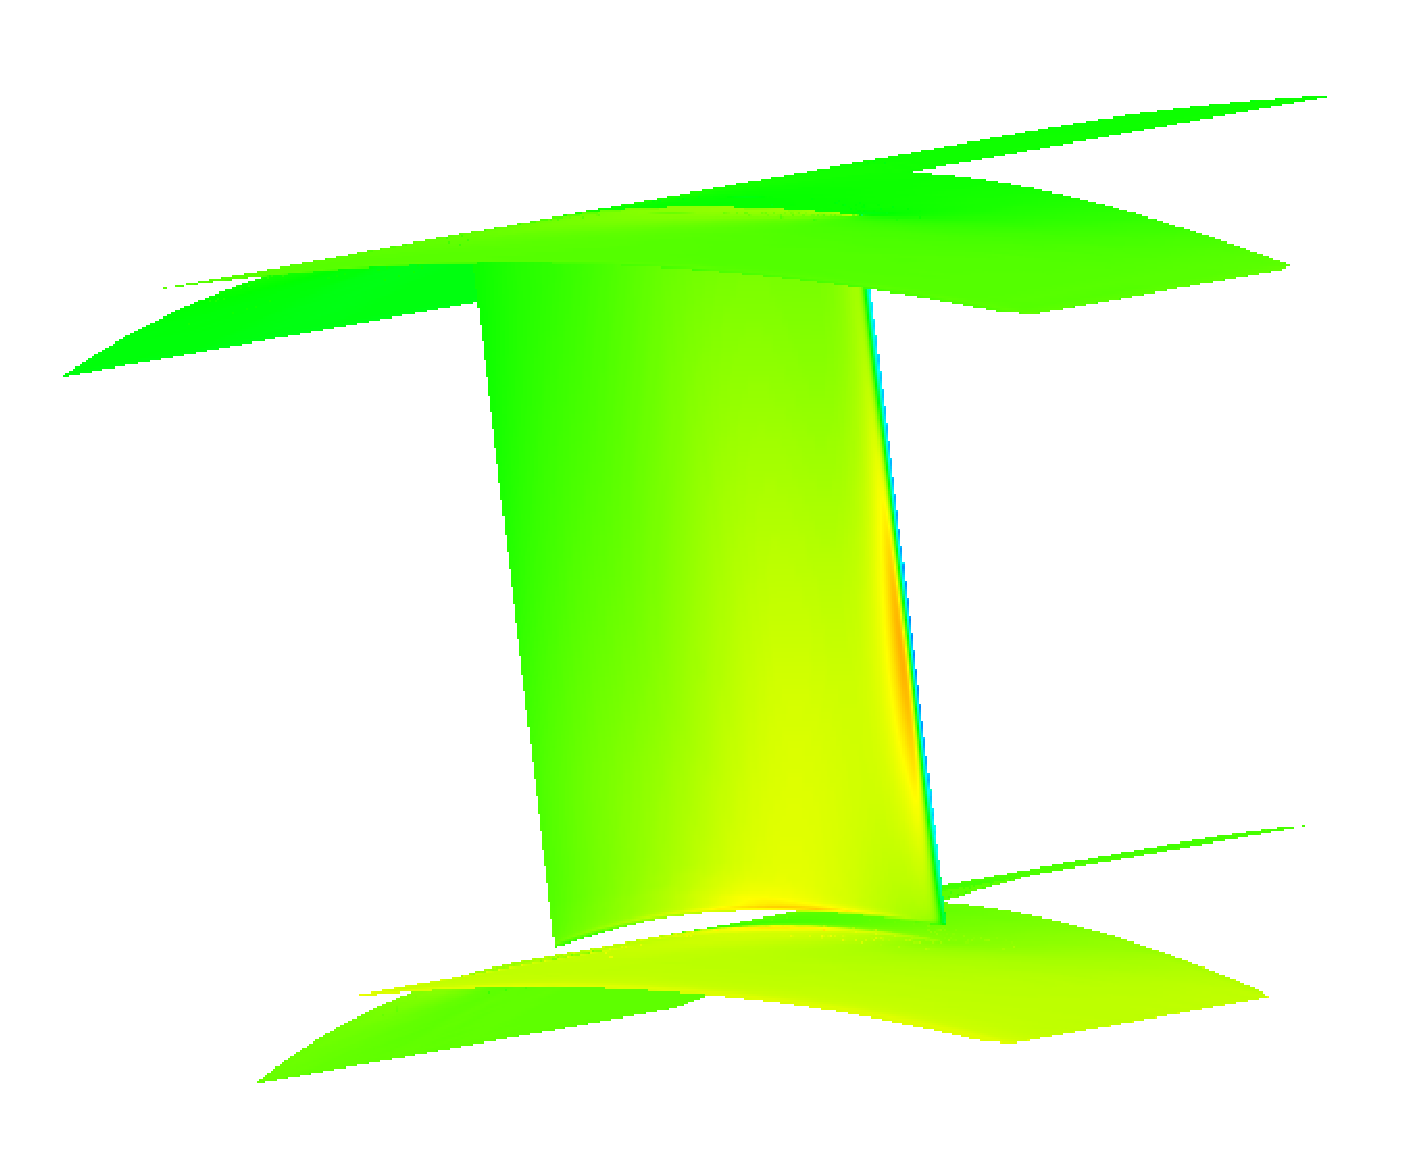
\includegraphics[width=.7\textwidth]{Optimal.eps}
%  \caption{Pressure contour over the optimal design.}
%  \label{res:ntua_blade:Optimal}
%\end{figure}

% ----------------------- end of thesis sub-document ------------------------
% ---------------------------------------------------------------------------
